\section{Algebra}
\label{sec:algebra}
\setlength{\textfloatsep}{5pt}% Remove \textfloatsep

In this section we describe the operators of \tg algebra.  The algebra
is compositional: all operators take a \tg or a pair of \tgs as input,
and produce a \tg.  Our algebra is based on the principles of snapshot
reducibility, which states that an operation should yield the same
result when applied to the temporal representation as it would if it
non-temporal version was applied separately to every snapshot state of
the temporal representation, and extended snapshot reducibility, which
requires that references to time can be used in the
operations~\cite{Dignos2012}.

%\subsection{Preliminaries}
%\label{sec:algebra:prelim}

\subsection{Maintaining integrity}
\label{sec:algebra:integrity}

Our algebra operates on \tgs, and so\eat{, in addition to keeping the
  data structure (and its constituent parts) coalesced,} we must
ensure that the result is a valid \tg.  One of the requirements of our
model is that each entity exists only once during any time instant
$t$.  To maintain this validity we introduce a {\em resolve} function.

\begin{definition}[Resolve function]
\eat{Let $((a_1,p_1),$ \\ $\ldots, (a_n,p_n))$ be a list of possible
  values of an attribute of a node or an edge along with their
  associated periods of validity.  A {\em resolve function} produces a
  single attribute value $a = resolve((a_1,p_1), \ldots, (a_n,p_n))$.}
Let $((a_l,p_l),(a_r,p_r))$ be a tuple of possible values of an
attribute of a node or an edge along with the associated validity
periods.  A {\em resolve function} produces a single attribute value
$a = resolve((a_l,p_l), (a_r,p_r))$.
\end{definition}

A resolve function can pick an arbitrary element, compute an average
for each property, put the values in a set, etc.  When applied over a
bag of values in a reduce fashion, a resolve function is a valid
aggregation function.  We support the standard \{ \insql{count} |
\insql{min} | \insql{max} | \insql{sum} \}, which have their customary
meaning.  We also support \{ \insql{any} | \insql{first} |
\insql{last} | \insql{set} | \insql{bag} \}, which are possible to
compute because properties being resolved have temporal information.
\insql{first} and \insql{last} refer to the value of an attribute with
the earliest/latest timestamp, while \insql{set} and \insql{bag}
associate a key an unordered collection of values with the set or bag
semantics (but do not keep the associated validity periods).  Finally,
we support \{ \insql{left} | \insql{right} \}, which select the
attribute of the left, resp. right, operand.  Other, more complex,
functions can be defined by the user.

\begin{lemma}
Let $\psi$ be an n-ary temporal operator on \tg.  If $\psi^T (\ttt)$
produces multiple possible attribute values for any entity at the same
time instant, it must also specify a resolve function to compute a
single valid attribute value.
\end{lemma}

\eat{ This objective informed our design of
  the algebra, e.g., we did not include some flavors of temporal
  aggregation because the result would be invalid.  Further, this
  objective informs the rewriting of applicable operations over the
  \ve representation.}  

Each operator in our algebra produces a valid \tg.  We note which
operators are known to uncoalesce the output, thus requiring
coalescing, require FK enforcement, or include the resolve function.

\subsection{Unary operators}
\label{sec:algebra:unary}

We introduce three basic unary operators: slice, subgraph, and map.
%\subsection{Slice}
%\label{sec:algebra:slice}

{\bf Slice.}  The unary {\em slice} operator, denoted $\tau_c (\ttt)$,
where $c$ is a time period, cuts a temporal slice from \ttt.  The
resulting \tg will contain nodes and edges whose period $p$ has a
non-empty intersection with $c$.  To evaluate $\tau_c (\tve)$, we
apply $\tau_c$ to each of the four constituent relations of \tve:
$\tau_c (\tv) = \{ (v, p \cap c)~~|~~(v, p) \in \tv \wedge
(\pred{c}{overlaps}{p} \vee \pred{c}{contains}{p}) \}$, and
analogously for each \te, \tav and \tae.

\eat{If $p.start < c.start$ or $p.end > c.end$ for some tuple $(g,
  p)$, then $p$ is trimmed to be within the boundaries of $c$: $\tau_c
  (\trg) = \{ (g, p \cap c)~~|~~(g, p) \in \trg \wedge
  (\pred{c}{overlaps}{p} \vee \pred{c}{contains}{p})\}$.  }
%

\eat{ 
In SQL, slice can be expressed as follows for $V$ (similarly for other
relations):}

\eat{\begin{small}
\begin{verbatim}
SELECT vid, a1, ..., an, greatest(estart, DATE ':date1'), 
       least(eend, DATE ':date2')
FROM V
WHERE eperiod OVERLAPS PERIOD (DATE ':date1', DATE ':date2')
\end{verbatim}
\end{small}}

Slice does not uncoalesce and does not require FK enforcement.  The
proofs for this and similar statements below are included in
Appendix~\ref{sec:app1}.

%\subsection{Temporal subgraph matching}
%\label{sec:algebra:subgraph}

{\bf Subgraph.}  Temporal subgraph matching is defined analogously to
subgraph matching in non-temporal graphs: it applies a predicate to
each node and edge of \tg. \eat{subgraph function $f$ to every
  representative graph of the input.  To ensure that a valid \tg is
  computed as a result of this operation, we restrict our attention to
  functions that compute a single subgraph of a given representative
  graph as a result: $\sigma_f (\trg) = \{ (g', p)~~|~~(g, p) \in \trg
  \wedge g' = f(g) \wedge$\\$V_{g'} \subseteq V_{g} \wedge E_{g'}
  \subseteq E_{g} \}$.}  Even more specifically, we focus on functions
that can be expressed as a pair of {\em conjunctive queries}
$\sigma_{C_V,C_E} (\ttt)$, where $C_V$ specifies predicates over the
vertices, and $C_E$ --- over the edges.  The predicates can be over
the attributes and also over the timestamps of the nodes/edges, to
support the extended snapshot reducibility.  (Computing arbitrary
subgraphs of an evolving graph is beyond the scope of this paper, and
we defer this to future work.)

$\sigma_{C_V,C_E} (\tve) = (\tv',\te',\tav',\tae') ~|~$ \\
$\tv' = \pi_{v,p} (\sigma_{C_{V1}} (\tv) \bowtie^T \sigma_{C_{V2}} (\tav)) \wedge \tav' = \sigma_{C_{V2}} (\tav)$ \\
$\te' = \pi_{v_1,v_2,p} (\sigma_{C_{E1}} (\te) \bowtie^T \sigma_{C_{E2}} (\tae)) \wedge \tae' = \sigma_{C_{E2}} (\tae)$.

\eat{Like other unary operators, $\sigma_{C_V, C_E} (\tve)$ follows the
outline of Algorithm~\ref{alg:op}.  Since $C_V$ and $C_E$ may involve
predicates over the attributes, we compute the join of the vertex
(resp. edge) relation with the corresponding attribute relation and
push selections:$\tv' = \pi_{v,p} (\sigma_{C_{V1}} (V) \bowtie
\sigma_{C_{V2}} (\tav))$ (line 1),$\te' = \pi_{v_1,v_2,p}
(\sigma_{C_{E1}} (E) \bowtie \sigma_{C_{E2}} (\tae))$ (line 2), $\tav'
= \sigma_{C_{V2}} (\tav)$ (line 3), $\tae' = \sigma_{C_{V2}} (\tae)$
(line 4).}

Subgraph does not uncoalesce, but does require FK enforcement for \tve.

%\subsection{Temporal map}
%\label{sec:algebra:project}

{\bf Map.}  The map operation applies user-defined map functions $M_V$
and $M_E$ to the vertices and edges of \tg.  To evaluate
$\map_{M_V,M_E} (\tve)$, we set $\tv'=\tv$ and $\te'=\te$, and compute
$\tav' = \map_{M_V}(\tav)$ and $\tae' = \map_{M_E}(\tae)$.

\eat{Temporal map iterates over the tuples of \trg, and applies the
user-specified map functions $M_V$ and $M_E$ to the vertices and edges
of each $g$: $\map_{M_V,M_E} (\trg) = \{(g', p)~~|~~(g,p) \in \trg
\wedge g'= \map_{M_V,M_E}(g)\}$.
}  

While map is an arbitrary user-specified function, there are some
common use cases.  Map can be used to remove vertex and edge
properties, as in projection.  In such cases we will use short-hand
notation similar to projection, listing the properties that we wish to
retain. For example, $\map_{M_V:{school},M_E:\emptyset} (\insql{T1})$
will keep only the school property of the vertices, and no properties
of the edges.  Another useful map operation eliminates duplicates in
the bag of a particular vertex or edge property.  \eat{It may also be
useful to flatten nested bags or aggregate multiple values of the same
property of a vertex or edge, e.g., compute a sum or an average
following temporal intersection or union
(Section~\ref{sec:algebra:join}).}

Map may uncoalesce \tav and \tae, but does not require FK enforcement.

\subsection{Binary operators}
\label{sec:algebra:binary}

We support the temporal versions of the three binary set operators
intersection ($\cap^T$), union ($\cup^T$), and difference
($\setminus^T$).

MORE HERE about how these three are not schema robust and require a resolver

\subsection{Temporal graph intersection}
\label{sec:algebra:join}

The binary temporal graph intersection operation $\trga \cap \trgb$
computes a temporal join~\cite{Gao2005} of \trga and \trgb with the
predicate $\trga.p \cap \trgb.p \neq \emptyset$, producing a tuple for
each pair of representative graphs for which time periods intersect:
$\trga \cap \trgb = \{(g_1 \cap g_2, p_1 \cap p_2)~|~((g_1, p_1) \in
\trga \wedge (g_2, p_2) \in \trgb \wedge p_1 \cap p_2 \neq \emptyset
\}$.  The result of $g_1 \cap g_2$ is computed by intersecting the
sets of vertices and of edges of the graphs~\cite{GraphTheory}.  For
each vertex and edge in the result, we compute a {\em union} of their
bags of properties.% \julia{Figure with example.}
%
Algorithm~\ref{alg:inter} presents the evaluation of $\tvea \cap
\tveb$. We compute temporal joins over \tv and \te (lines 1, 2).  We
then compute \tav' and \tae' with temporal outer joins of the
corresponding relations (lines 3, 4).  Finally, we enforce foreign key
constraints on \te', \tav' and \tae' (lines 5, 6).

\begin{algorithm}[b]
\caption{Temporal graph intersection in \tve.}
\begin{algorithmic}[1]
%\REQUIRE $\tvea (\tv_1;\te_1;\tav_1;\tae_1), \tveb (\tv_2;\te_2;\tav_2;\tae_2)$.\\
\REQUIRE $\tvea, \tveb$.\\
\STATE $\tv' = \tv_1 \Join^T_v \tv_2$\\ 
\STATE $\te' = \te_1 \Join^T_{v_1,v_2} \te_2$\\ 
\STATE $\tav' = \cl (\pi_{v,p,\tav_1.a \cup \tav_2.a}\tav_1 \fullouterjoin^T_v \tav_2)$\\
\STATE $\tae' = \cl (\pi_{v_1,v_2,p,\tae_1.a \cup \tae_2.a}\tae_1 \fullouterjoin^T_{v_1,v_2} \tae_2)$\\
%\STATE $\tae' = \pi_{a_1 \cap a_2}(\tae_1 \Join^T \tae_2)$\\
\STATE enforce foreign keys on $\tav'$ w.r.t. $\tv'$\\ 
\STATE enforce foreign keys on $\tae'$ w.r.t. $\te'$\\ 
\RETURN new $\tve (\tv';\te';\tav';\tae')$\\
\end{algorithmic}
\label{alg:inter}
\end{algorithm}

\begin{figure}
%\centering
\begin{subfigure}[b]{0.4\columnwidth}
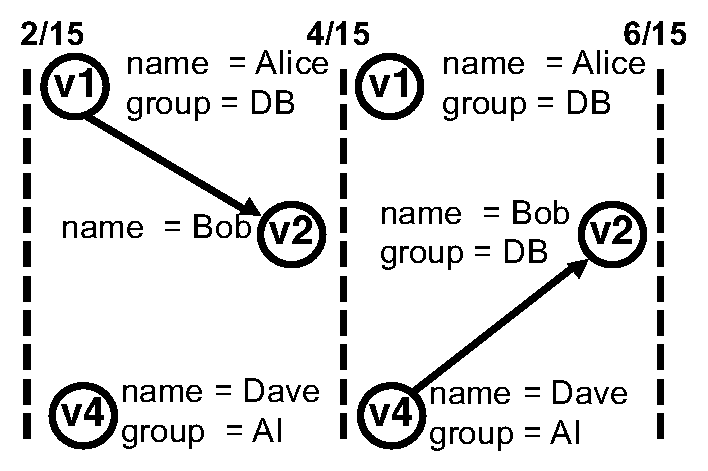
\includegraphics[width=1.35in]{figs/T2_graphs.pdf}
\caption{T2.}
\vspace{-0.2cm}
\label{fig:tg_t2}
\end{subfigure}
\begin{subfigure}[b]{0.5\columnwidth}
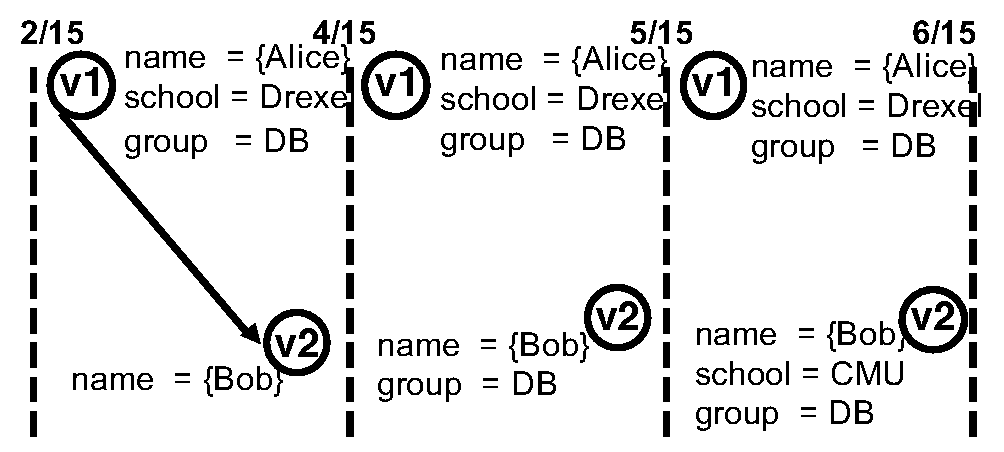
\includegraphics[width=2in]{figs/T1_inter_T2.pdf}
\caption{$T1 \cap T2$.}
\vspace{-0.2cm}
\label{fig:tg_inter}
\end{subfigure}
\caption{Temporal intersection.}
\label{fig:intersect}
\vspace{-0.2cm}
\end{figure}

Figure~\ref{fig:intersect} illustrates temporal intersection of \tg
T2, shown in Figure~\ref{fig:tg_t2}, with T1 in our running example.
Period $[2/15, 4/15)$ is computed as a result of the join of $[2/15,
    5/15)$ in T1 and [$2/15, 4/15)$ in T2.  Only the vertices and
      edges present in both \tgs are produced, thus eliminating $v_3$
      and $v_4$.  Notice the result of attribute bag union with
      duplicates for some keys.  These can be resolved by a subsequent
      \insql{map} based on the domain requirements.

{\bf Intersection may uncoalesce \tve and \trg.}  While temporal join over
coalesced temporal relations does not uncoalesce, as shown
in~\cite{DBLP:conf/vldb/BohlenSS96}, it is followed by a projection,
which does uncoalesce.  For example, consider a simple \tg $T_2$
that consists of only 1 vertex $v_1$ with attribute $(name:Alice)$ and
no edges and exists for the period $[1/14, 5/15)$.  The
  intersection of $T_2$ with \insql{T} in Figure~\ref{fig:tg_rg}
  produces the same graph with vertex $v_1$ for each period of
  intersection $[1/15, 2/15), [2/15, 5/15)$, which must be coalesced.

{\bf Intersection requires FK enforcement for \tav and \tae but not
  for \te.}  \eat{The proof for this is similar to the one for
  \insql{slice}. } Consider an edge $\te(v_1, v_2, p^e) \in \te'$ and
one of the corresponding vertices $\tv(v_1, p^v) \in \tv'$ computed in
Algorithm~\ref{alg:inter}.  To violate the FK constraint on \te',
there must exist a time instant $t \in p^e \wedge t \not\in p^v$.  But
that is not possible, since by definition of temporal join $p^e$
exists in both $\te_1$ and $\te_2$, and $\tve_1$ and $\tve_2$ are
valid \tgs.  To see why we need to enforce FK for $\tav'$, consider
again the example above with $T \cap T_2$.  The temporal outer join of
$\tav_1$ and $\tav_2$ will produce a tuple for period [1/14, 1/15)
  with the attribute $(name:Alice)$ from $\tav_2$.  Clearly this tuple
  violates the FK constraint because we do not have any vertices in
  $\tv'$ prior to 1/15.  Similarly for $\tae'$.

\subsection{Temporal graph union}
\label{sec:algebra:outerjoin}

The binary temporal graph union operation $\trga \cup \trgb$ computes
a temporal full outer join~\cite{Gao2005} of \trga and \trgb on the
predicate $\trga.p \cap \trgb.p $. For tuples $(g_1, p_1) \in \trga$
and $(g_2, p_2) \in \trgb$ for which $p_1 \cap p_2 \neq \emptyset$, we
compute $(g_1 \cup g_2, p_1 \cap p_2)$.  The result of $g_1 \cup g_2$
is computed by taking a {\em union} of the sets of vertices and of
edges of the graphs~\cite{GraphTheory}.  For each vertex and edge in
the result, we compute a {\em union} of their bags of properties.
Tuples from \trga (resp. \trgb) for which there does not exist a tuple
in \trgb (resp. \trga) for part or all of the validity period are
included in the result of the full outer join. 
%\julia{Figure with example.}
\eat{
 $\trg_1 \cup \trg_2 = \{ (g, p) | (g_1, p_1) \in \trg_1 \wedge (g_2,
p_2) \in \trg_2 \wedge ((g = g_1 \cup g_2 \wedge p = p_1 \cap p_2
\wedge p_1 \cap p_2 \neq \emptyset) \vee (g = g_1 \wedge p = p_1 - p_2
\wedge \nexists p \in \trg_2 = p_1 - p_2) \vee (g = g_2 \wedge p = p_2
- p_1 \wedge \nexists p \in \trg_1 = p_2 - p_1))\}$.  Similar to
temporal intersection, temporal union is essentially an outer
theta-join of $\trg_1$ and $\trg_2$ with a $p_1 \cap p_2$ predicate.
We use the standard graph union definition based on set theory, which
computes unions of the vertex and edge sets from the two
operands~\cite{GraphTheory}.}
%
Algorithm~\ref{alg:union} presents the evaluation of $\tvea \cup
\tveb$.  We compute temporal outer joins over the corresponding \tv,
\te, \tav and \tae.

\begin{algorithm}[t]
\caption{Temporal graph union in \tve.}
\begin{algorithmic}[1]
\REQUIRE $\tvea, \tveb$.\\
\STATE $\tv' = \tv_1 \fullouterjoin^T_v \tv_2$\\
\STATE $\te' = \te_1 \fullouterjoin^T_{v1,v2} \te_2$\\
\STATE $\tav' = \cl (\pi_{v,p,\tav_1.a \cup \tav_2.a}\tav_1 \fullouterjoin^T_v \tav_2)$\\
\STATE $\tae' = \cl (\pi_{v_1,v_2,p,\tae_1.a \cup \tae_2.a}\tae_1 \fullouterjoin^T_{v1,v2} \tae_2)$\\
\RETURN new $\tve (\tv';\te';\tav';\tae')$\\
\end{algorithmic}
\label{alg:union}
\end{algorithm}

\eat{\begin{algorithm}
\caption{Temporal graph union in \tve.}
\begin{algorithmic}[1]
\REQUIRE $\tve_1 (\tv_1, \te_1, \tav_1, \tae_1), \tve_2 (\tv_2, \te_2, \tav_2, \tae_2)$.\\
\STATE $\tv' = \tv_1 \fullouterjoin^T \tv_2$\\
\STATE $\te' = \te_1 \fullouterjoin^T \te_2$\\
\STATE $\tav' = \pi_{a_1 \cup a_2}(\tav_1 \fullouterjoin^T \tav_2)$\\
\STATE $\tae' = \pi_{a_1 \cup a_2}(\tae_1 \fullouterjoin^T \tae_2)$\\
\RETURN new $\tve (\tv', \te', \tav', \tae')$\\
\end{algorithmic}
\label{alg:union}
\end{algorithm}
}

{\bf Union may uncoalesce \tve and \trg.}  The logic here is similar
to the case with temporal intersection.  Because we produce a single
graph for each time period by computing a union of $g_1$ and $g_2$, a
form of projection, the result may be uncoalesced.  For example,
consider a simple \tg $T_2$ that consists of a single graph equal to
the first representative graph of \insql{T} in Figure~\ref{fig:tg_rg}
valid for a period of $[12/14, 5/15)$.  The same representative graph
  will be produced for period $[12/14, 1/15)$ and $[1/15, 2/15)$ and
      must be coalesced.  $\tv'$ and $\te'$ are coalesced since they
      are computed with a temporal
      join~\cite{DBLP:conf/vldb/BohlenSS96}.  However, $\tav'$ and
      $\tae'$ are computed with a join followed by a projection, which
      does uncoalesce.  Thus we apply the coalescing operation on
      lines 3 and 4.

{\bf Union does not require FK enforcement for \tve.} Temporal full
outer join produces a vertex tuple for all periods in $\tv_1$ and
$\tv_2$.  If $\tve_1$ and $\tve_2$ are valid graphs, then 
referential integrity holds for $\te'$, $\tav'$ and $\tae'$.

\eat{\begin{definition}[Union] Union of $TG1\ \cup\ TG2$ = $\{v, e: v
    \in TG1.V$ or $v \in TG2.V$ or $v(vid$, $f_1(a_{11}$, $a_{21})$,
    \ldots, $f_n(a_{1n}, a_{2n})$, $period(least(p_1, p_2),
    greatest(p_1, p_2)))$, $e \in TG1.E$ or $e \in TG2.E$ or $e(vid1,
    vid2, g_1(b_{11}, b_{21}), \ldots, g_m(b_{1m}, b_{2m})$,
    $period(least(p_1, p_2), greatest(p_1, p_2))) \}$, where each $f$,
    respectively $G$, is an aggregation function over one vertex,
    respectively edge, attribute where the values intersect over some
    period $p$.
\label{def:union}
\end{definition}}

\eat{\begin{figure*}
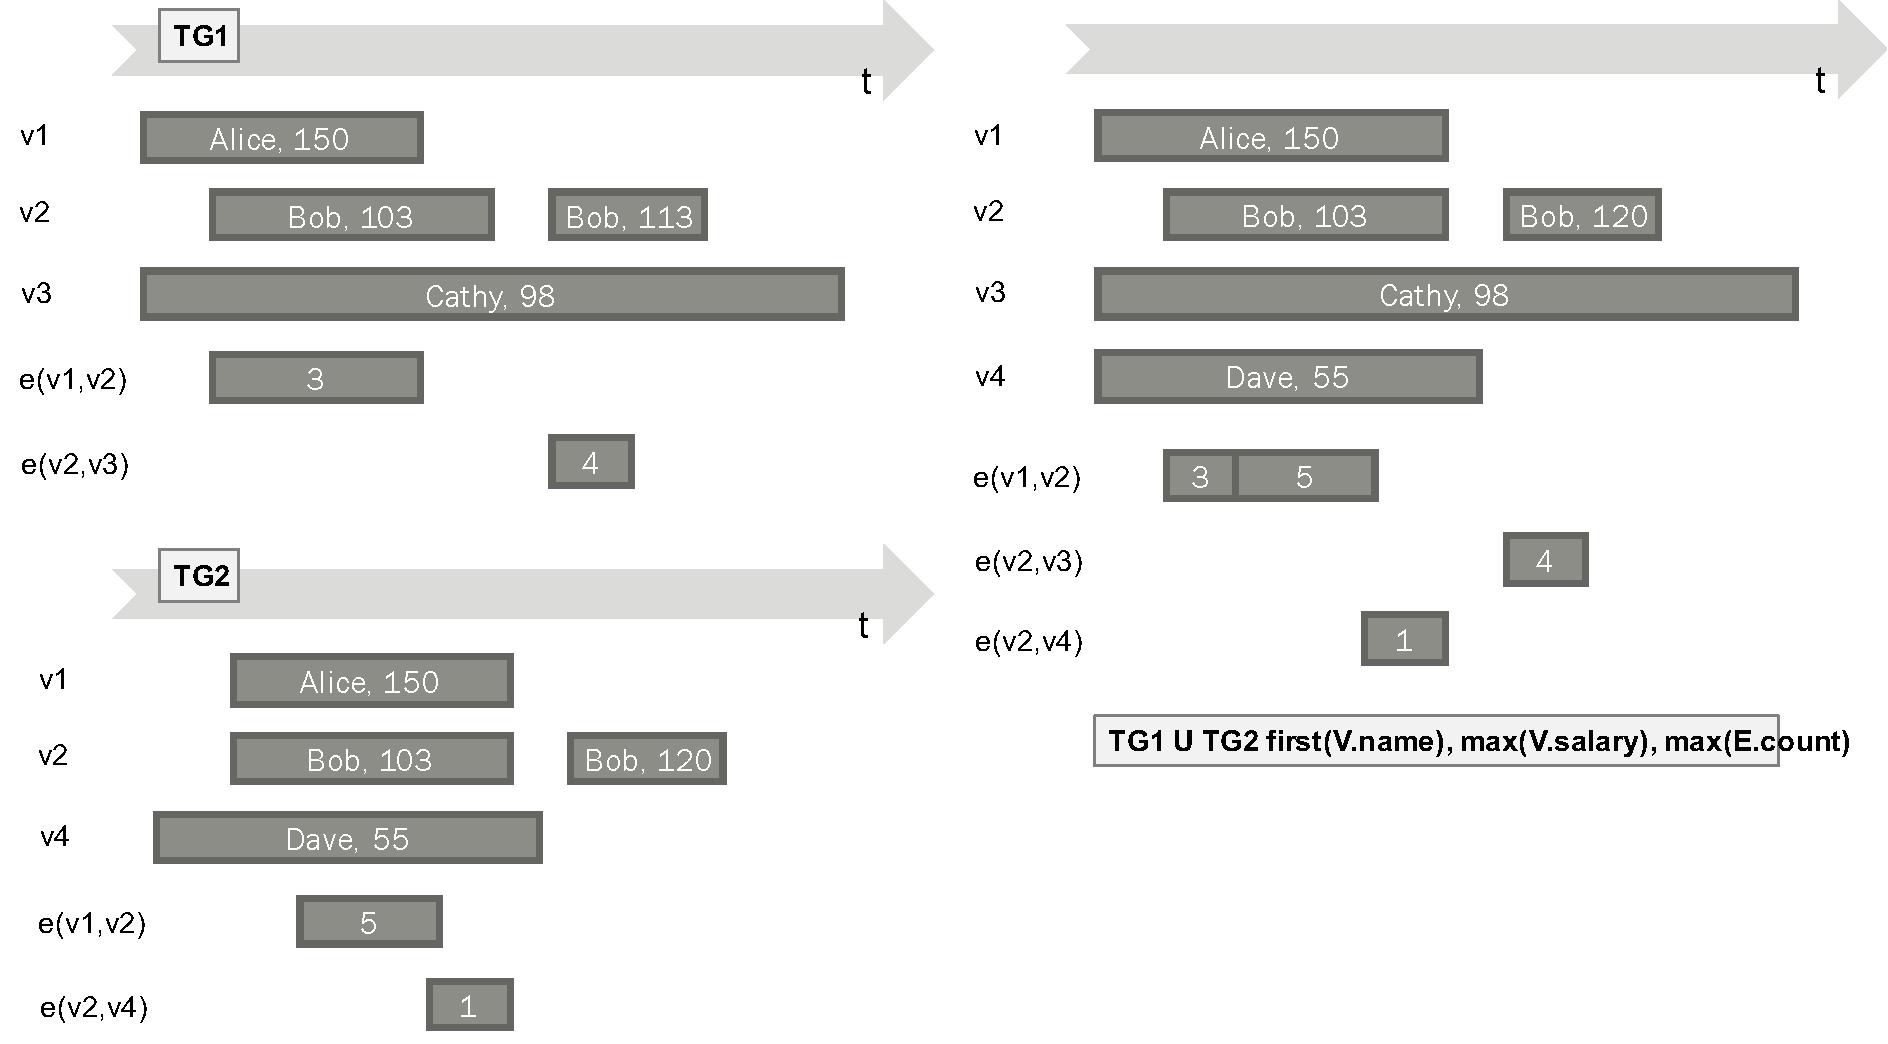
\includegraphics[width=6.5in]{figs/union.pdf}
\caption{Union of TG1 and TG2.}
\label{fig:union}
\end{figure*}}

\eat{In other words, union of two \tgs is simply all vertices and edges
from both \tgs, with vertex/edge attributes decided by specified
aggregation functions for each period where both values are present,
with coalescing.  Figure~\ref{fig:union} illustrates this concept.}

\eat{Similarly, intersection of two \tgs is an intersection of
vertices/edges of two graphs, with values for each overlapping
attribute computed by a specified aggregate function.}

\subsection{Temporal graph difference}
\label{sec:algebra:diff}

The binary temporal graph difference operation $\trga \setminus \trgb$
computes a temporal left outer join~\cite{Gao2005} of \trga and \trgb
on the predicate $\trga.p \cap \trgb.p$.  For tuples $(g_1, p_1) \in
\trga$ and $(g_2, p_2) \in \trgb$ for which $p_1 \cap p2 \neq
\emptyset$, we compute $(g_1 \setminus g_2, p_1 \cap p_2)$.  The
result of $g_1 \setminus g_2$ is computed by taking a {\em set
  difference} of the sets of vertices and of edges of the graphs.  For
each vertex and edge in the result, we compute a {\em union} of their
bags of properties.  Tuples in \trga for which there does not exist a
tuple in \trgb for part or all of the validity period are included in
the result of the left outer join.

Algorithm~\ref{alg:diff} presents the evaluation of $\tvea \setminus
\tveb$.  We compute temporal left outer joins over the corresponding
\tv and \te (lines 1,2).  We then compute $\tav'$ and $\tae'$ with
temporal outer joins of the corresponding relations (lines 3, 4).
Finally, we enforce foreign key constraints on $\te'$, $\tav'$, and
$\tae'$ (lines 5, 6).

\begin{algorithm}[b]
\caption{Temporal graph difference in \tve.}
\begin{algorithmic}[1]
\REQUIRE $\tvea, \tveb$.\\
\STATE $\tv' = \tv_1 \leftouterjoin^T_v \tv_2$\\ 
\STATE $\te' = \te_1 \leftouterjoin^T_{v_1,v_2} \te_2$\\ 
\STATE $\tav' = \cl (\pi_{v,p,\tav_1.a \cup \tav_2.a}\tav_1 \fullouterjoin^T_v \tav_2)$\\
\STATE $\tae' = \cl (\pi_{v_1,v_2,p,\tae_1.a \cup \tae_2.a}\tae_1 \fullouterjoin^T_{v_1,v_2} \tae_2)$\\
\STATE enforce foreign keys on $\tav'$ w.r.t. $\tv'$\\ 
\STATE enforce foreign keys on $\tae'$ w.r.t. $\te'$\\ 
\RETURN new $\tve (\tv';\te';\tav';\tae')$\\
\end{algorithmic}
\label{alg:diff}
\end{algorithm}

%maybe figure here

{\bf Difference may uncoalesce \tve and \trg.}  The logic here is
similar to the temporal union and intersection cases above.  Because
we produce a single graph for each time period by computing a $g_1
\setminus g_2$, a form of projection, the result may be uncoalesced.
For example, consider a simple \tg $T_2$ as above, i.e. equal to the
first representative graph of \insql{T} in Figure~\ref{fig:tg_rg}
valid for a period of $[2/15, 7/15)$.  The same representative graph
  will be produced for period $[5/15, 6/15)$ and $[6/15, 7/15)$ and
      must be coalesced.  As with union and intersection, $\tv'$ and
      $\te'$ are coalesced since they are computed with a temporal
      join~\cite{DBLP:conf/vldb/BohlenSS96}.  However, $\tav'$ and
      $\tae'$ are computed with a join followed by a projection, which
      does uncoalesce.  Thus we apply the coalescing operation on
      lines 3 and 4.

{\bf Difference requires FK enforcement for \tav and tae but not \te.}
The proof for this is the same as for intersection and we will not
repeat it.

\subsection{Aggregation}
\label{sec:algebra:agg}

Aggregation is a common graph operation that can be used to compute
simple properties such as in-degrees of nodes or more complex ones
such as a set of places that all close friends have visited in the
past year.  Aggregation is denoted $\gamma_{C_V,C_E,A_V}$, where $C_V$
is a predicate over the source and destination nodes of the edge,
$C_E$ is a predicate over the edge itself, and $A_V$ is an aggregation
function.  The result is a new graph $\gamma_{C_V,C_E,A_V} (\tve) = \tve' = (\tv', \te', \tav', \tae') | \tv' = \tv \wedge \te' = \te \wedge \forall (v', p', a') \in \tav' \exists$. TODO



\subsection{Node creation}
\label{sec:algebra:create}

We argued in the introduction that it is interesting and insightful to
analyze an evolving graph at different levels of granularity.  For
example, the user may want to aggregate multiple consecutive
representative graphs into a single representative graph, coarsening
the granularity, or to predefine temporal resolution and look at the
graph at that scale, irrespective of whether this resolution happens
to be finer or coarse than the natural evolution rate of the graph.
For this, we introduce a node creation operator which is similar to
the {\em moving window temporal aggregation} in temporal relational
algebra.  Our approach is inspired by stream aggregation work
of~\cite{Li2005}, adopted to graphs, and by generalized quantifiers
of~\cite{Hsu1995}.

Node creation is denoted $_{G_V}create_{W,Q_V,Q_E,A_V,A_E}
(\ttt)$,\\ where $G_V$ are the grouping attributes, $W$ is the window
specification, $Q_V$ and $Q_E$ are vertex and edge quantifiers, and
$A_V$ and $A_E$ are the optional aggregation functions.  It produces a
consolidated evolving graph with specific temporal granularity.

{\em Grouping attributes} $G_V$ are vertex properties by which
vertices are aggregated into new entities, similar to \insql{GROUP BY}
clause in SQL.  Since node creation requires new identifiers, the
combination of the grouping properties can be used in a mechanism
equivalent to a Skolem function.  The simplest, default grouping
attribute is the $vid$ of the vertex.

{\em Window specification} $W$ is of the form
$n~\{unit|\insql{changes}\}$, where $n$ is an integer, and $unit$ is a
time unit, e.g., $10~min$, $3~years$, or any multiple of the usual
time units.  Window specification of the form $n~\insql{changes}$
defines the window in terms of change over \trg.\eat{ (which may be
  computed from the \tve representation, see
  Section~\ref{sec:model:switch}).}  For example,
$W=3~\insql{changes}$ will aggregate sequences of 3 representative
graphs into 1.  Window boundaries are computed left-to-right, i.e.,
from least to most recent.  The right-most window may correspond to
fewer than $n$ representative graphs from the input.
%
Our window specification by change is similar to slide-by-row window
in stream aggregation~\cite{Li2005}.  Note that, because \tg algebra
is compositional, we do not support node creation with
overlapping windows, because it does not produce a valid \tg.  To see
why this is so, consider applying a sliding window of 3 months range
with 1 month slide to graph \insql{T} in Figure~\ref{fig:tg_rg}.  We
would produce the following set $(g_1, [1/15, 4/15)), (g_2, [4/15,
    7/15)), (g_3, [7/15, 10/15))$, which clearly violates the
      temporally coalesced requirement in
      definition~\ref{tg_abstract}.  

Similar to~\cite{Li2005} we support creation simultaneously by time
and by non-temporal attributes (e.g., vertex properties).  If the
window specification is one change, then the operation devolves into
pure structural reduce or node creation, as classified by
Wood~\cite{Wood2012}.  If the grouping attribute is the vertex $vid$,
then the operation is purely temporal, with no structural aspect.

{\em Quantifiers} $Q_V$ and $Q_E$ are of the form \{ \insql{all} |
\insql{most} | \insql{at least} $n$ | \insql{exists} \}, where $n$ is
a decimal representing the percentage of the time during which an
entity (vertex or edge) existed, relative to the duration of the
window. These are useful for producing different kinds of
representative graphs.  For example, to produce representative graphs
with only strong connections over a volatile evolving graph, we may
want to only include vertices that span the entire time window
($Q_V=\insql{all}$), and edges that span a large portion of the window
($Q_E=\insql{most}$).
 
The optional {\em aggregation functions} $A_V$ and $A_E$ compute new
values for vertex and edge properties representative of
the whole window, e.g., $A_V=\insql{any}(name), \insql{last}(school)$
and $A_E=\insql{sum}(cnt)$.
%
 
Key-value pairs for vertex and edge properties for which no aggregation
functions are specified, are collected into a list corresponding to the
entity in the result.  These can be subsequently transformed with
temporal map (Section~\ref{sec:algebra:project}).
 
Temporal aggregation over \tve follows the outline of
Algorithm~\ref{alg:op}, but requires an additional step, and is
revisited in Algorithm~\ref{alg:agg_ve}.
%
We compute group periods based on window specification in line
1.  Next, as part of $_{G_V}create_{P,Q_V}(\tv)$ computation, we assign
each tuple from \tv to a period (this requires
splitting), group vertices by $G_V$ and evaluate $Q_V$ on each group.
Only groups for which $Q_V$ evaluates to true are retained.  Edges are
processed similarly by $_{G_V}create_{P,Q_E}(\te)$ on line 3.  Note that
when $G_V$ is anything besides $vid$, we need edge triplets in order
to compute new source and destination ids of each edge.  Lines 4 and 5
compute $_{G_V}create_{P,A_V}(\tav)$ and $_{G_V}create_{P,A_E}(\tae)$,
respectively, by computing a group for each vertex or edge within the
period, and applying the aggregate functions over each group. \eat{ It
  is possible but inconvenient to express the operations on lines
  2---5 in temporal SQL because each vertex, edge or attribute tuple
  in the result of $create_{P}$ may belong to multiple periods.}

Node creation over \trg is computed by first calculating time periods
from $W$ and \trg, and then reducing and combining the representative
graphs directly.

\begin{algorithm}[t!]
\caption{Node creation in \tve.}
\begin{algorithmic}[1]
\REQUIRE \tve (\tv;\te;\tav;\tae), window specification $W$, vertex
quantifier $Q_V$, edge quantifier $Q_E$, vertex aggregate function
$A_V$, vertex aggregate function $A_E$.\\
\STATE $P = \textsf{computePeriods}(W, \tv, \te, \tav, \tae)$\\
\STATE  $\tv' = \cl (_{G_V}create_{P,Q_V}(\tv))$\\
\STATE  $\te' = \cl (_{G_V}create_{P,Q_E}(\te))$\\
\STATE  $\tav' = \cl (_{G_V}create_{P,A_V}(\tav))$\\
\STATE  $\tae' = \cl (_{G_V}create_{P,A_E}(\tae))$\\
\STATE  follow steps 5-7 of Algorithm~\ref{alg:op}\\
%\STATE  enforce foreign keys on $\te'$ w.r.t. $\tv'$\\
%\STATE  enforce foreign keys on $\tav'$ w.r.t. $\tv'$\\
%\STATE  enforce foreign keys on $\tae'$ w.r.t. $\te'$\\
\RETURN new $\tve (\tv';\te';\tav';\tae')$\\
\end{algorithmic}
\label{alg:agg_ve}
\end{algorithm}

Figure~\ref{fig:tg_agg1} illustrates node creation by time
($W=3~\textsf{months}$), and Figure~\ref{fig:tg_agg2} --- by change
($W=3~\textsf{changes}$).  Figure~\ref{fig:tg_agg3} illustrates
structural reduce only ($W=1~\textsf{change}$), and
Figure~\ref{fig:tg_agg4} both structural and temporal
($G_V=\textsf{school}, W=3~\textsf{months}$).  All four are applied to
\insql{T1} in our running example, and list the same aggregation
quantifiers (\insql{all} for vertices and \insql{exists} for edges)
and aggregate functions (\insql{first} for vertex and edge
properties).  $v_2$ is present in the result in
Figure~\ref{fig:tg_agg1} starting at $4/15$ because it did not exist
for the entirety of the first window, while in
Figure~\ref{fig:tg_agg2} it is produced starting $6/15$.  In
Figure~\ref{fig:tg_agg3} vertices $v1$ and $v3$ are aggregated into a
single new vertex $v1$ representing the institution.  A subsequent
\insql{map} operation to produce a new name attribute and a count of
people would produce a more meaningful final result.


%\julia{add brief explanation.}
\eat{Note that $(v_2, [4/15, 7/15))$ is present in the result in
  Figure~\ref{fig:tg_agg1} because $v_2$ exists for the entire period
  in the input \insql{T1}.  Further, because vertex properties took on
  values $(Bob, Penn)$ and $(Bob, CMU)$ during this period, but $(Bob,
  Penn)$ was temporally earlier, this value is used.  This is in
  contrast to only $(Bob, CMU)$ being associated with $v_2, [7/15,
    10/15)$.}
\eat{Next, consider the result of $create_2$, and note that, while $v_2$
 was present for part of $[1/15, 5/15)$, it was not there during the
   entirety of the period, and so is not included into the result.
   Edge $e(v_1, v_2)$ is absent during $[1/15, 5/15)$, because one of
     the vertices it connects ($v_2$) does not exist.}

\eat{
\begin{figure}[t!]
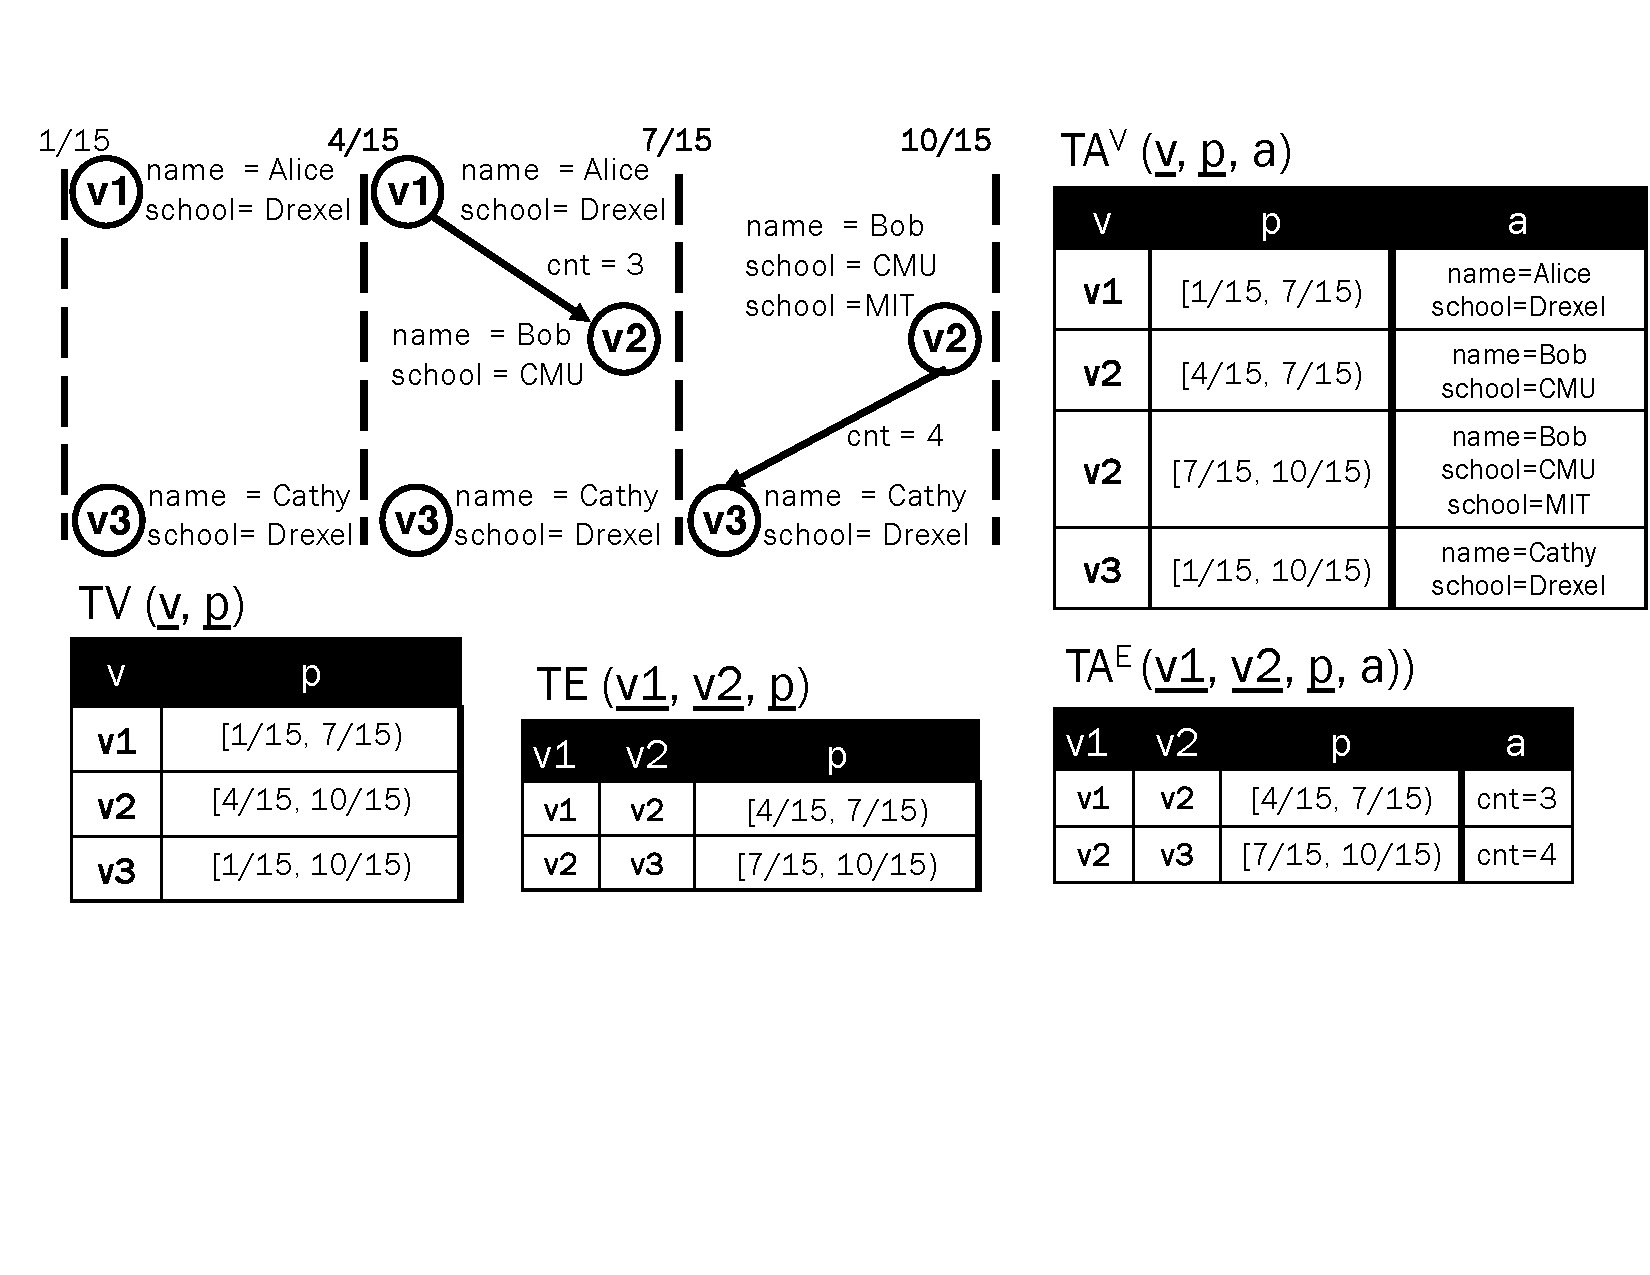
\includegraphics[width=3.5in]{figs/agg1.pdf}
\caption{Aggregation of \insql{T1} by time:
  $W=3~\textsf{months}$, $Q_V=\insql{all}$, $Q_E=\insql{exists}$,
  $A_V=\insql{first}$, $A_E=\insql{first}$.}
\vspace{-0.2cm}
\label{fig:tg_agg1}
%\vspace{-0.2cm}
\end{figure}
}
\eat{
\begin{figure}[t!]
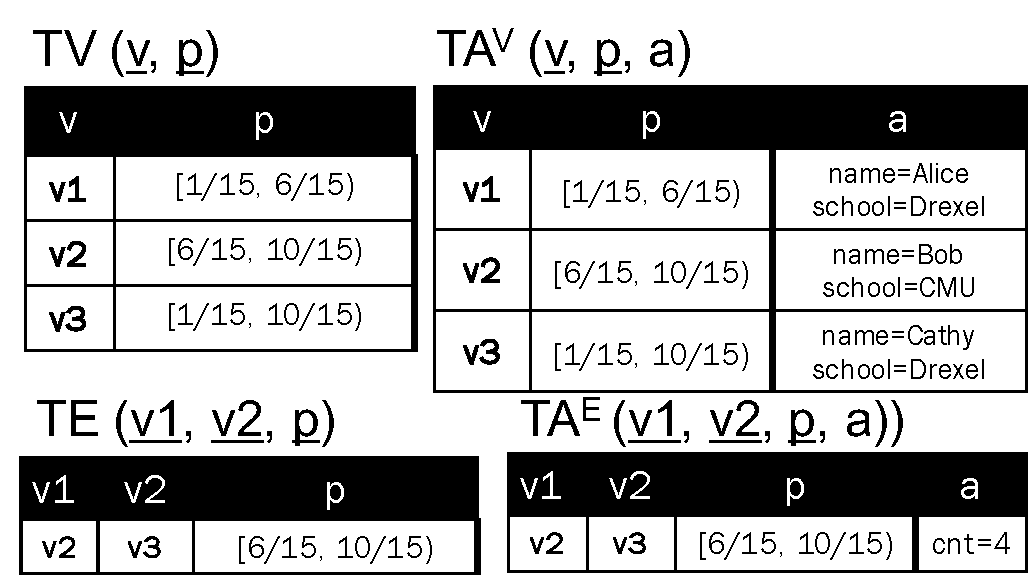
\includegraphics[width=3in]{figs/agg2.pdf}
\caption{Aggregation of \insql{T1} by change:
  $W=3~\textsf{changes}$, $Q_V=\insql{all}$, $Q_E=\insql{exists}$,
  $A_V=\insql{first}$, $A_E=\insql{first}$.}
\vspace{-0.2cm}
\label{fig:tg_agg2}
%\vspace{-0.2cm}
\end{figure}
}

\begin{figure*}[t]
%\centering
\begin{subfigure}[b]{0.5\textwidth}
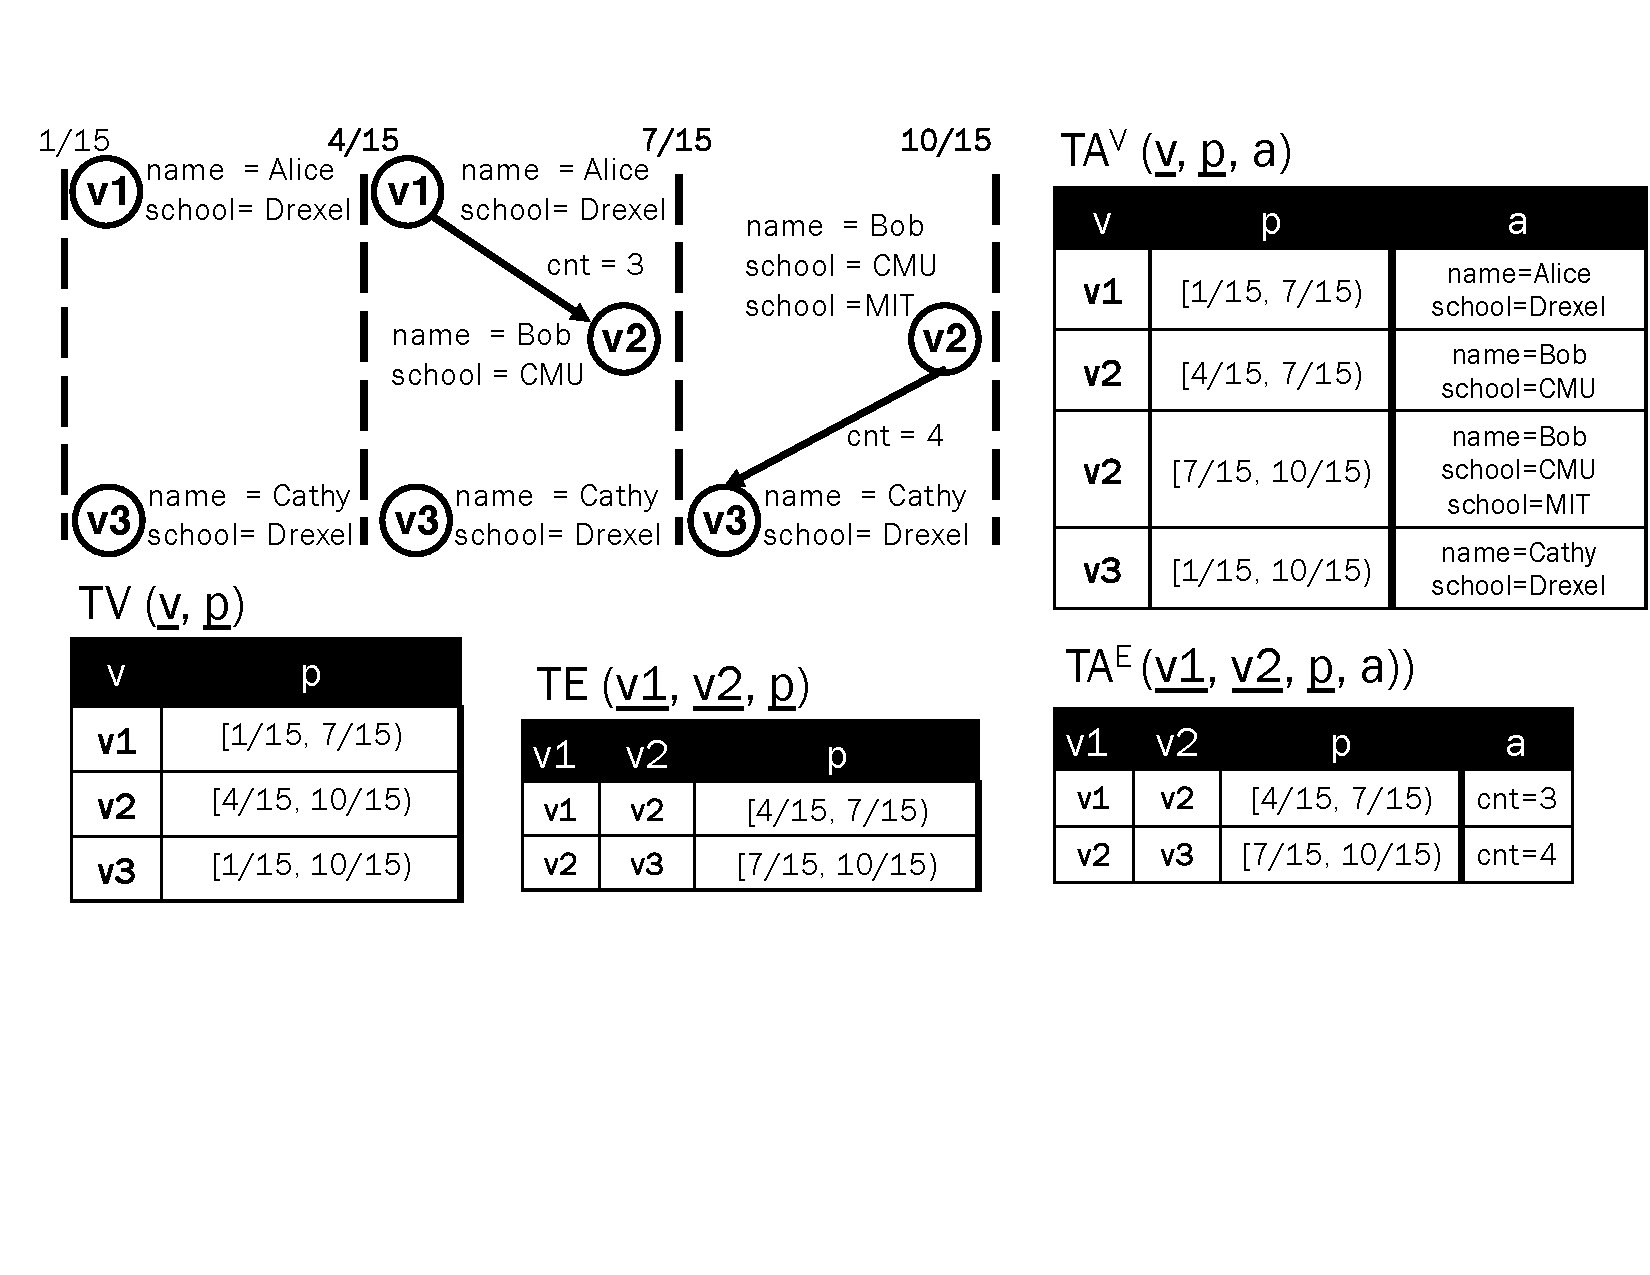
\includegraphics[width=3.5in]{figs/agg1.pdf}
\caption{Aggregation of \insql{T1} by time:
  $W=3~\textsf{months}, G_V=\textsf{vid}$.}
\label{fig:tg_agg1}
\end{subfigure}
\begin{subfigure}[b]{0.4\textwidth}
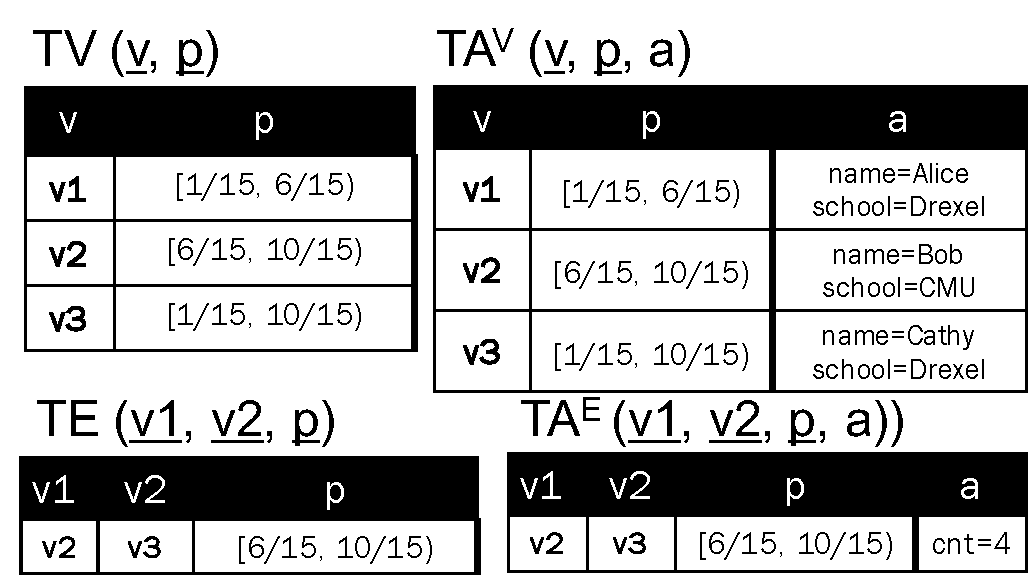
\includegraphics[width=3in]{figs/agg2.pdf}
\caption{Aggregation of \insql{T1} by change:
  $W=3~\textsf{changes}, G_V=\textsf{vid}$.}
\label{fig:tg_agg2}
\end{subfigure}
\begin{subfigure}[b]{0.5\textwidth}
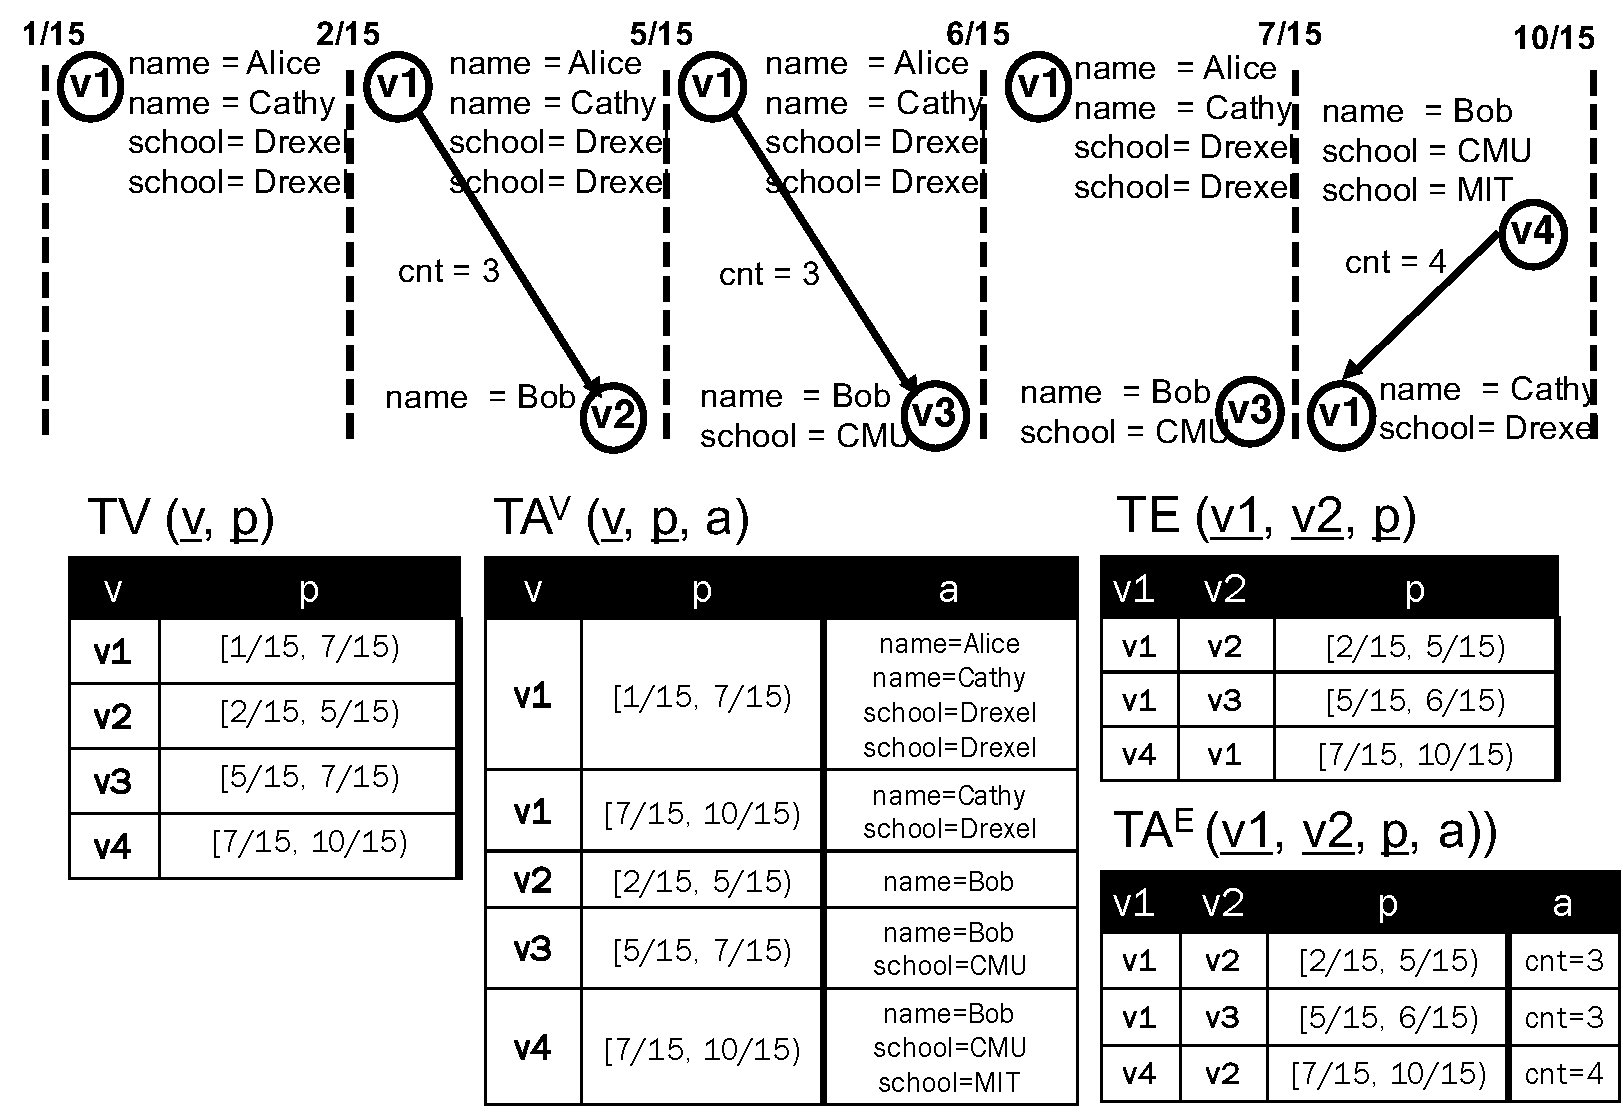
\includegraphics[width=3.5in]{figs/agg3.pdf}
\caption{Aggregation of \insql{T1} grouped by attribute:
  $W=1~\textsf{change}, G_V=\textsf{school}$.}
\label{fig:tg_agg3}
\end{subfigure}
\begin{subfigure}[b]{0.4\textwidth}
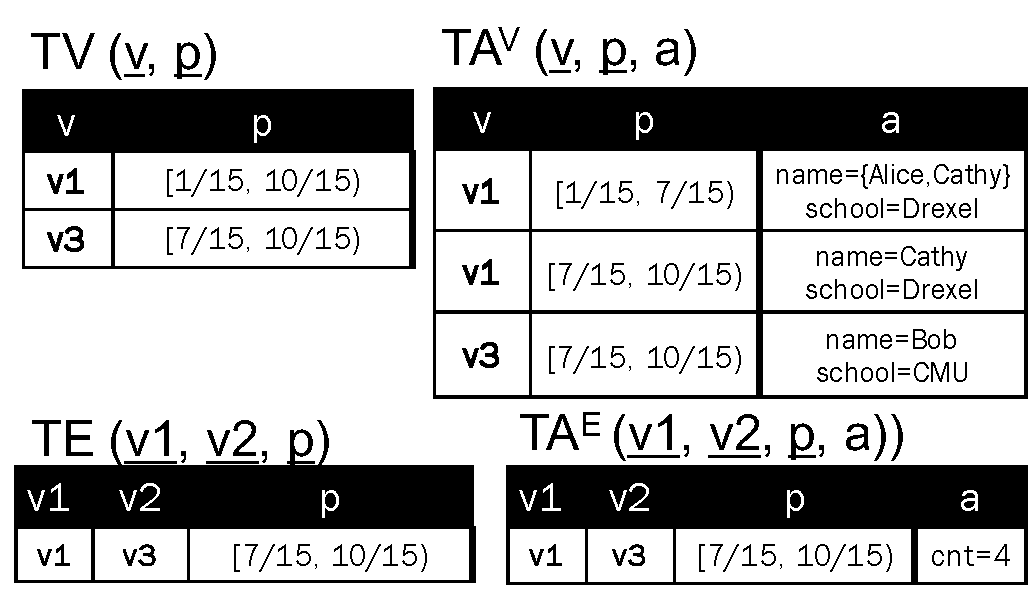
\includegraphics[width=3in]{figs/agg4.pdf}
\caption{Aggregation of \insql{T1} by time with grouping:
  $W=3~\textsf{months}, G_V=\textsf{school}$.}
\label{fig:tg_agg4}
\end{subfigure}
\caption[]{Aggregation, $Q_V=\insql{all}$, $Q_E=\insql{exists}$,
  $A_V=\insql{first}$, $A_E=\insql{first}.$}
\label{fig:tg_agg}
\vspace{-0.5cm}
\end{figure*}

{\bf Node creation may uncoalesce \tve and \trg.}  Consider
\insql{T} that consists of only 1 vertex $v_1$ and no edges, and
suppose that $v_1$ exists during the odd months of the year.  \tv
contains $(v_1, [1/16, 2/16)), \ldots,$ $(v_1, [11/16,12/16))$, for
    which time periods do not meet and so these tuples cannot be
    coalesced.  Next consider $\tve'$ in the result of
    $create_{W=2~months, Q_V=exists,Q_E=all}(T)$.  This relation will
    contain $(v_1, [1/16, 3/16)), \ldots,$ $,(v_1, [11/16,1/17))$ ---
        one tuple per input tuple, all tuples meet and so \tv' must be
        coalesced.  A similar argument holds for, \te, \tav, \tae,
        \trg.

{\bf Node creation requires FK enforcement for \tve.}  As
illustrated in Figure~\ref{fig:tg_agg1}, $(v_1,v_2,[1/15,4/15))$ is
  absent from $\te'$ because, although this edge was present in \tv
  for part of the period, and so meets the condition
  $Q_E=\insql{exists}$, vertex $(v_2,[1/15,5/15))$ is absent from
    $\tv'$.

We now give an analysis of whether FK enforcement is required, by
considering the relationship between vertex and edge aggregation
quantifiers $Q_V$ and $Q_E$.  Recall that we support quantifiers
\insql{all}, \insql{most}, \insql{at least} $n$, and \insql{exists},
and observe that they can be translated to a threshold on the
percentage of the time during which an entity (vertex or edge)
existed, relative to the duration of the window specification: $t = 1$
for \insql{all}, $t > 0.5$ for \insql{most}, $t > 0$ for
\insql{exists} and $t > n$ for \insql{at least} $n$.  Let us refer to
the vertex threshold as $t_V$, and to the edge threshold as $t_E$.  If
an entity's existence meets the threshold, it will be retained in the
result.

FK enforcement is only required if $t_V > t_E$.  To see why, consider
an interval $w$ which is one of the windows computed based on
specification $W$.  We produce an edge $(v_1, v_2, w)$ iff $\exists
\{(v_1, v_2, p_1),\ldots,(v_1, v_2, p_k)\} \in
\te~~|~~(\bigcup_{i=1}^k p_i \cap w) / w > t_E$.  According to
Definition~\ref{def:tg:c1}, if the input graph is valid then we must
also produce $(v_1, w)$ and $(v_2, w)$ if $t_V \leq t_E$, since vertex
periods are supersets of edge periods.  However, if $t_V > t_E$, we
may not produce a vertex that meets $t_E$ but does not meet the
greater $t_V$, as we showed with the example above.

\eat{FK enforcement is only required if $t_V$ is stricter
than $t_E$.  To see why, consider 2 cases.  (1) Suppose that $t_V \leq
t_E$.  To violate FK constraint, we must produce edge $(v_1, v_2, p)
\in \te'$ and not produce vertex $(v_1, p) \in \tv'$.  This edge
$(v_1, v_2)$ must have been valid during at least $t_E$ portion of p
in \te.  If our input is valid, then there must exist both $v_1$ and
$v_2$ in \tv during at least $t_E$ portion of p to pass the FK
constraint.  Since $t_E$ is at least as large as $t_V$, we will
produce both $(v_1, p)$ and $(v_2, p)$.  (2) $t_V > t_E$.  The proof
here is similar to above.  If we produce edge $(v_1, v_2, p) \in
\te'$, then there must be both $v_1$ and $v_2$ in \tv that exist
during at least $t_V$ portion of p.  However, since $t_V$ is larger
than $t_E$, we may not produce a vertex in \tv' that meets $t_E$ but
does not meet the greater $t_V$.  In that case the edge is violating
the FK constraint.}

\eat{ Our aggregation quantifiers are inspired by generalized
  quantifiers of~\cite{Hsu1995} with n-place delimiters.  $Q(R)$ as a
  Boolean-valued function of a relation''~\cite{Hsu1995}.  A
  quantifier contains an n-place determiner, e.g., ``at least one
  vertex in each window for each group'' is a 2-place determiner
  quantifier.  \tg algebra supports determiners from the set
  $\{at\ least\ one, all, most, at\ least\ n\}$, where $n$ is an
  integer representing a ratio.  $all$ is a usual universal quantifier
  that in standard SQL can be achieved with the use of two \insql{NOT
    EXISTS}.}

\eat{Aggregation in relational algebra produces results for each grouping
irrespective of how many results there are, unless a \insql{HAVING}
restriction is applied.  The quantification over the aggregation
results in evolving graphs is useful for producing different kinds of
representative graphs.  For example, to produce a representative graph
with only strong connections over a volatile evolving graph, we want
to restrict results to those edges that span the entire window or a
large subset of that window.  For this purpose we introduce
quantifiers.}

\eat{
The second observation is that it is necessary to enforce referential
integrity.  Consider a pair of relations $R_i, R_j \in T_{VE}$, such
that there is a foreign key on $R_j$ referencing $R_i$, and consider
the counterparts of these relations $R'_i = \sigma_{c_i} R_i$ and $R'_j
= \sigma_{c_j} R_j$.  If the selection condition on $R_i$ is trivial
(i.e., $R_i = \sigma_{c_i} R_i$), then referential integrity will hold
on $R_i, R_j$.  However, if $c_i$ removes some tuples from $R_i$, then
it becomes necessary to identity tuples in $R'_j$ for which there is
no counterpart in $R'_i$ and delete them.}

\eat{
Recall that a \tg is a pair of coalesced temporal SQL relations, with
an integrity constraint that ensures that an edge exists at a time
when both vertices it connects also exist.  We start by investigating
the behavior of our model under a standard definition of temporal
relational algebra operators applied to $V$, $E$ or both in
Section~\ref{sec:algebra:rel}.  We then present the novel operations
of \tg algebra (Section~\ref{sec:algebra:graph}).  The main challenge
in both sub-section is understanding whether and when to coalesce $V$
and $E$, and how to efficiently enforce the integrity of the data
structure.}

%\subsection{Relational algebra operators over $V$ and $E$}

\eat{$V$ and $E$ are valid-time temporal relations, and we adopt (and
adapt) the semantics of period-based temporal
algebra~\cite{DBLP:conf/vldb/BohlenSS96} to our setting. }

\eat{1) Apply operation to V
2) Apply operation to E
3) Coalesce V if necessary
4) Coalesce E is necessary
5) Enforce integrity constraint}

\eat{Temporal selection $\sigma_c V = \{ \langle v, p, a_1, \ldots, a_n
\rangle | c(\langle v, p, a_1, \ldots, a_n \rangle) \}$ returns a
subset of the tuples in $V$. Note that the selection condition $c$ is
an arbitrary Boolean condition that may also include predicates on
$p$.  }

\eat{When evaluated over coalesced input relations, temporal selection,
temporal Cartesian product and temporal negation preserve coalescing.}

\eat{
\begin{definition}[Selection]
Temporal and structural selection on $TG$ is a selection on the
attributes of $V$ and $E$, including entity periods.  $\sigma_{a
  \theta c}(TG)$, where $a$ are attributes of $V$ and/or $E$,
including periods, $\theta$ is a binary operation in the set $\{<,
\leq, =, \neq, \geq, >\}$, and $c$ is a value constant.
\label{def:selection}
\end{definition}}

\eat{Temporal and structural selection are supported by the same selection
operator and can be used together.  For example, one could select a
sub-graph in an evolving co-citation network of only authors whose
names start with letter A, over the past decade.  Because of the
constraint on $E$, even if the structural selection is only on
attributes of $V$, only edges connecting selected vertices are
retained.  Neither deduplication nor coalescing is required as a
post-operation.  Note that temporal selection and slice are different
because temporal selection does not modify entity periods, only
selects some of them.}

\eat{In SQL, selection can be expressed as a regular selection on V,
followed by a selection on E with integrity constraint enforced.}

\eat{\begin{definition}[Projection]
Projection on $TG$ is projection on attributes of $V$ and $E$ with
coalescing, i.e. \\$\Pi vid, p, a_1, \ldots, a_n(V); \Pi vid_1, vid_2,
p, b_1, \ldots, b_m(E)$. 
\label{def:projection}
\end{definition}}

\eat{\begin{definition}[Slice]
The unary operation \op{slice}, denoted $\sigma_{[start, end)}
  \insql{T}$ is a selection operation that includes...}

\eat{Slice on $TG$ is a selection on periods of $V$ and $E$ such that
$slice_{[a,b)}(TG) = \{t': t \in TG$, $t(p).overlaps(period(a,b)), t'
  = fit(t, period(a,b))\}$ and $fit(t, period(a,b))$ shortens the
  entity period $p$ to be within $[a,b)$.
\label{def:slice}
\end{definition}}

\eat{In SQL, slice can be expressed as follows for $V$
(similarly for $E$):}

\eat{\begin{small}
\begin{verbatim}
SELECT vid, a1, ..., an, greatest(estart, DATE ':date1'), 
       least(eend, DATE ':date2')
FROM V
WHERE eperiod OVERLAPS PERIOD (DATE ':date1', DATE ':date2')
\end{verbatim}
\end{small}}

%\subsection{Temporal aggregation}

\eat{Now that we have the window semantics and quantification defined, we
can define the aggregation operation over an evolving graph $TG$.}

\eat{It is often useful to analyze aggregate behavior of an evolving graph
over some coarser time period.  For example, a union of all
vertices/edges over 1 month is representative of that graph during
that month.  Analysis of aggregate behavior can lead to deeper insight
than of a snapshot.  For example, a co-authorship network DBLP is very
sparse --- one can only publish so many papers in any given month ---
on a daily or even monthly level of granularity, but can show
community formation and affiliation when aggregated over multiples of
years.  From this perspective, an evolving graph is a sequence of
representative graphs over consecutive arbitrary-length periods.}

\eat{
\begin{definition}[\tg Aggregation]
An {\em aggregation} operation over $TG$ is a function \\ $G_1, G_2,
\ldots, G_n, W, Q g f_1(A_1), f_2(A_2), \ldots, f_m(A_m)(TG)$, where
each $G_i$ is a grouping attribute from $TG$ with the exception of
$p$; $W$ is the window specification; $Q$ is a generalized quantifier
specification for vertices and edges on the coverage of the window;
each $F_i$ is an aggregation function; and each $A_i$ is an attribute
name from $TG$.
\label{def:agg}
\end{definition}}

\eat{This definition is similar to the regular relational algebra
aggregation definition, with the addition of the window specification
and the restriction of grouping attributes to exclude the time
periods.  However, both $V$ and $E$ relations are aggregated by the
same operation and the constraint on $E$ to contain only those
vertices that exist in $V$ is maintained.  The aggregation defined
this way allows to aggregate graphs structurally, temporally, or in
combination.  To aggregate only temporally, the grouping attribute
must be $vid$ for $V$ and $(vid1, vid2)$ for $E$.  To aggregate only
structurally, the window specification must be by 1 change.  Observe
that aggregation by 1 change with grouping by id is a no-op, and in
fact the sequence of representative graphs on the source data is equal
to the deduplicated sequence of snapshots.}

\eat{The quantifier is applied to the coverage of the window period
  within each grouping.  For example, to construct the persistent
  edges graph from the example above, we use the $all$ quantifier over
  the $E$ relation.  Only the edges that span the duration of the
  window period are produced.  Since the universal quantification is
  very restrictive, $most$ and $at\ least\ n$ quantifiers are more
  appropriate in some aggregations, especially over long windows.  To
  obtain a stable 1-month graph over an evolving network connections
  graph, we may ask for connections that exist in at least 90\% of the
  period.}

\eat{Remember that the schema for $V$ has a $(vid, p)$ primary key.  Any
aggregation operation must produce both a valid $vid$ and valid time
interval for each tuple.  We produce a $vid$ by using the hash of the
grouping variables to maintain temporal consistency.  The time
interval is produced by the window extent from the window
specification. Similarly for $E$.}

\eat{The aggregation functions over the selected graph attributes are used
to compute the new value representative of the whole window.  We
support the standard set $\{count, min,$ $max, sum, average\}$, as
well as $\{any, first, last, list\}$.  $first$ and $last$ refer to
first/last non-null value in the window and are possible because the
aggregating tuples have the time dimension, and the ties are decided
arbitrarily.  $count$ is the count of the number of distinct values
over the aggregation window.  Additional aggregation functions can be
defined by the user.}

\eat{\begin{figure*}
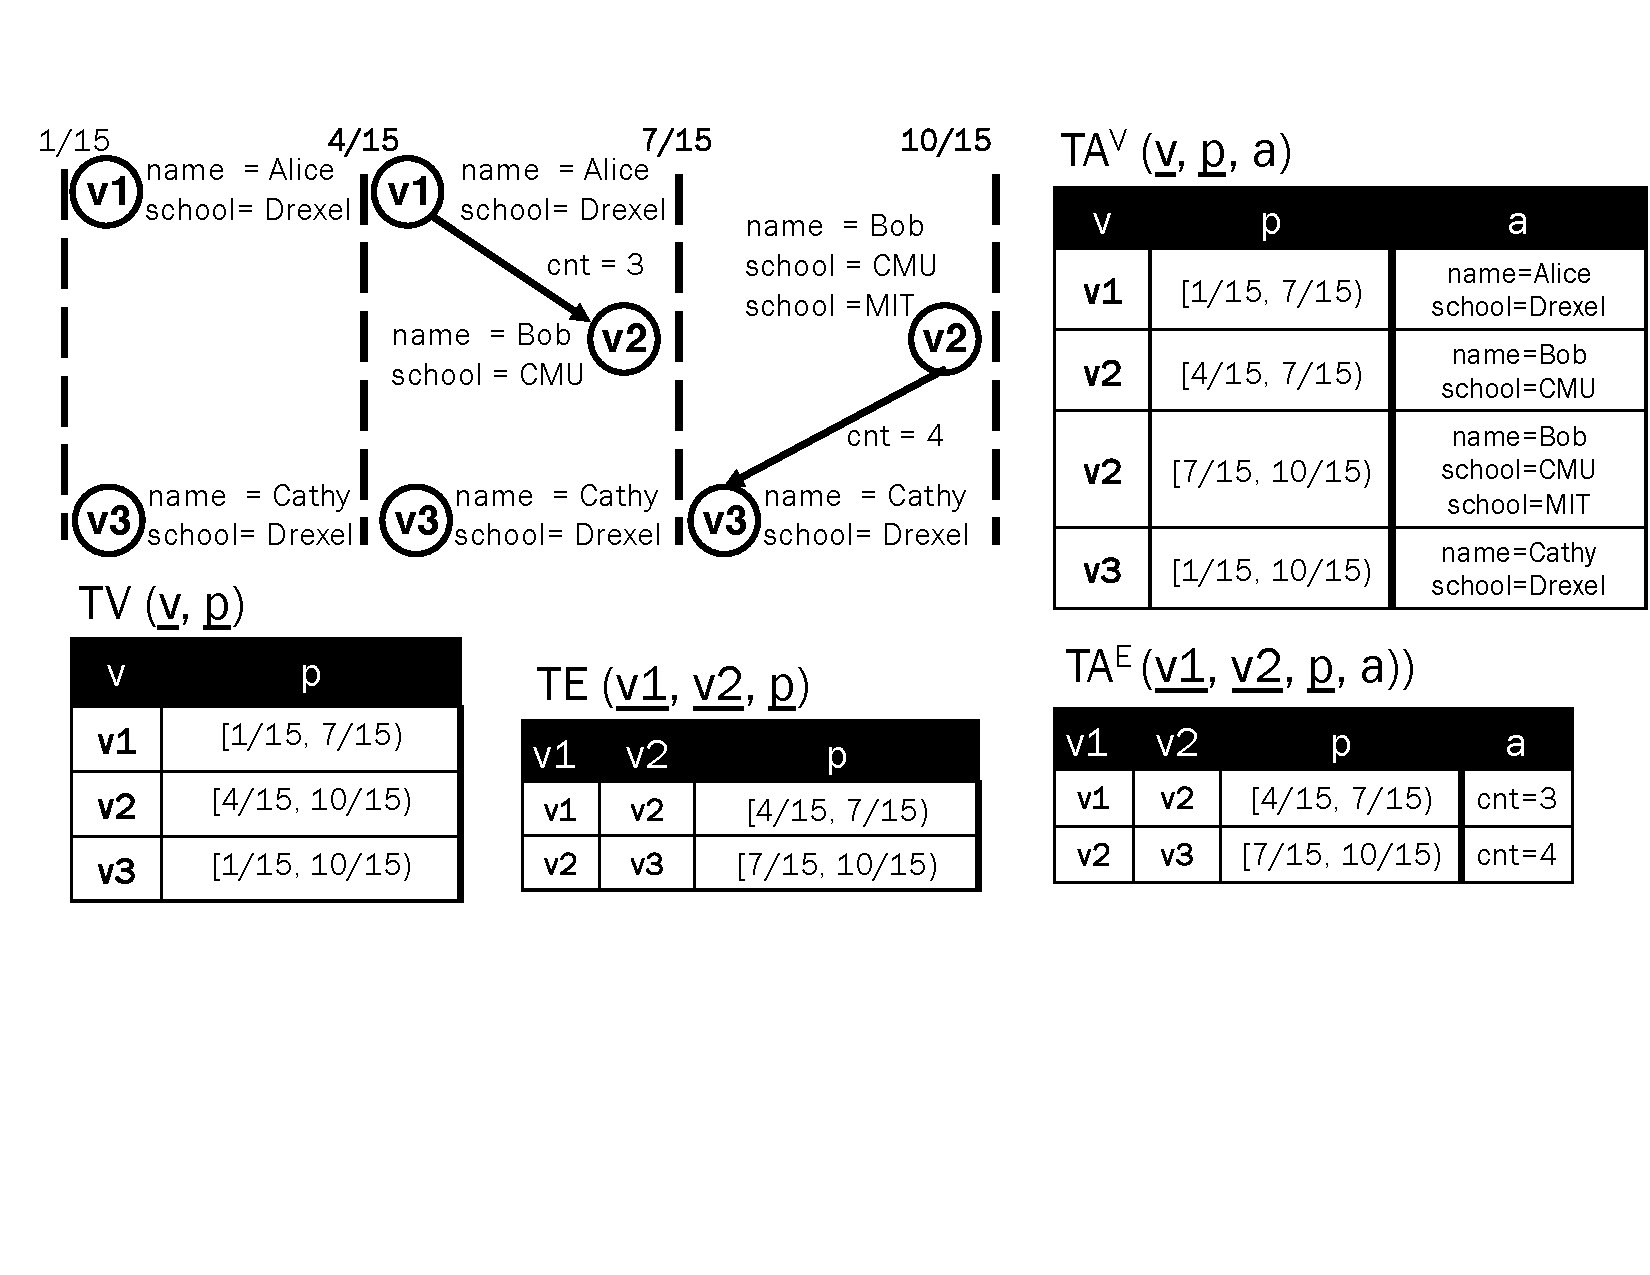
\includegraphics[width=6.5in]{figs/agg1.pdf}
\caption{1-month window aggregation with grouping by id, with
  existential vertex/edge quantifier.  Structure only.}
\label{fig:agg1}
\end{figure*}
}

\eat{An example in Figure~\ref{fig:agg1} shows a small \tg and a result of
aggregation by 1 month on that graph with $at\ least\ one$ quantifier,
with group by id.}

\subsection{Transitive closure}
\label{sec:algebra:closure}

TODO


\eat{So far we have defined the operations in our temporal graph
  algebra.  Next we define another class of non-algebraic operations
  on evolving graphs that are nevertheless very useful: analytics.}

\eat{\vera{What I think we are leaving out: difference, structural
  aggregation (new entity creation), graph joins and products (maybe?
  graph joins are weird), more general select (with time in predicate
  and/or path predicates), reverse/transpose.}}
